\documentclass[12pt, titlepage]{article}
\usepackage[utf8]{inputenc}
\usepackage[margin=1.0in]{geometry}

\title{Balloon Catheter Training Device User Manual}
\author{Nam Tran\\ Biomedical Engineering\thanks{Undergraduate}, The George Washington University}
\date{November 2018}

\usepackage[english]{babel}
\usepackage{graphicx}
\usepackage{float}
\usepackage{forest}

\usepackage[parfill]{parskip}

\begin{document}

\maketitle

\section{Introduction}
Balloon catheterization in this case is used for transvenous cardiac pacing, often utilised in the emergency department. This user manual describes a step-by-step narrative for using the device, referencing the objectives, functions, and user stories determined for this product. All user stories, objectives, and functions can be found in "Backgrounds, Vision, and Needs" \cite{backgroundreport}. They are also summarised in the appendix at the end of the document.


\section{Narrative}

\subsection{Installation}

All necessary software for the training model are packaged on the provided USB drive. The USB drive is organised as follows:

\begin{forest}
  for tree={
    font=\ttfamily,
    grow'=0,
    child anchor=west,
    parent anchor=south,
    anchor=west,
    calign=first,
    edge path={
      \noexpand\path [draw, \forestoption{edge}]
      (!u.south west) +(7.5pt,0) |- node[fill,inner sep=1.25pt] {} (.child anchor)\forestoption{edge label};
    },
    before typesetting nodes={
      if n=1
        {insert before={[,phantom]}}
        {}
    },
    fit=band,
    before computing xy={l=15pt},
  }
[Balloon-Catheter
  [Installation
    [GUI-Install.msi]
  ]
  [Documentation
    [User-Manual.pdf]
    [Licenses.pdf]
  ]
]
\end{forest}

Prior to use, the software should be installed by running the installation files found under "Installation". As of the writing of this manual, the only necessary software to download is the GUI software for interfacing with the training model.

\subsection{Training Set-Up}

Prior to the training exercise, the instructor should have the device connected to the school's wireless network (similar to a wireless printer). On the training room control computer, open the GUI software and mirror it to the training room's hospital monitor. This process can be assisted by the school's IT department. The GUI will request that you choose which training model to display for (in case of multiple training exercises being conducted at once). The GUI will indicate when the training model is calibrated and ready for use.

\begin{figure}[H]
\centering
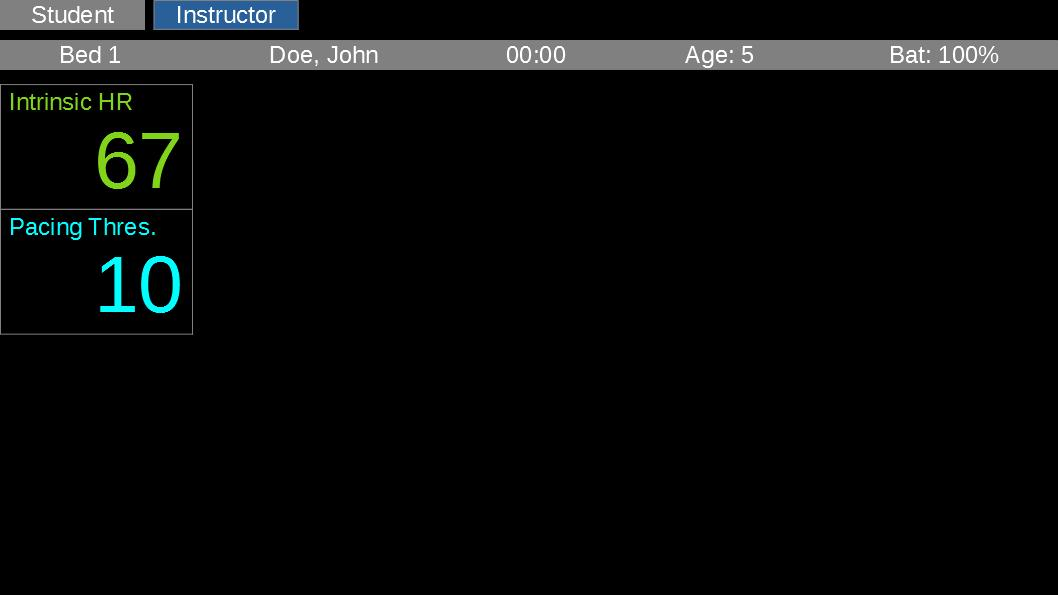
\includegraphics[scale=0.5]{gui-teacher}
\caption{Instructor GUI screen for setting simulation options}
\label{fig:teacher}
\end{figure}

At any time, the instructor is able to input a starting intrinsic heart rate for the training model to display (Figure \ref{fig:teacher}). This will automatically show on the GUI when the catheter is inserted into the model. The instructor is also able to set a pacing threshold for the pacer to reach at any time as well.

\subsection{General Use}
You will begin the training using a balloon catheter and pacer provided by your instructor. These are outside of the scope of what this training device includes. From there, follow the instructor's direction on the actual medical procedure. This procedure is standard and outside of the scope of operating our training device specifically.

\begin{figure}[H]
\centering
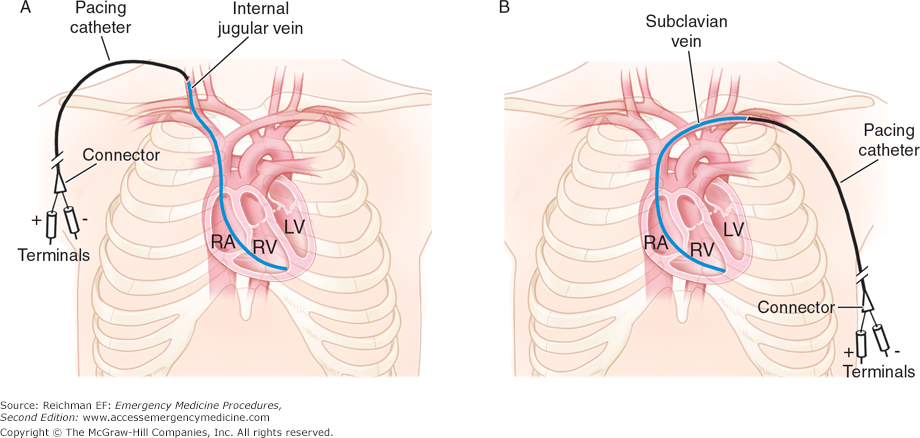
\includegraphics[scale=0.5]{transvenous}
\caption{Catheter path through the jugular vein and subclavian vein \cite{reichman2013emprocedures}}
\label{fig:procedure}
\end{figure}

The training device will not provide feedback until the catheter has been inserted into the jugular vein (For reference, please see Figure \ref{fig:procedure}). As specified in User Stories 1 and 2, Objectives 2, 4, and 6, and Functions 1, 2, and 3; the simulation room monitor will display an ECG (Figure \ref{fig:student}).

\begin{figure}[H]
\centering
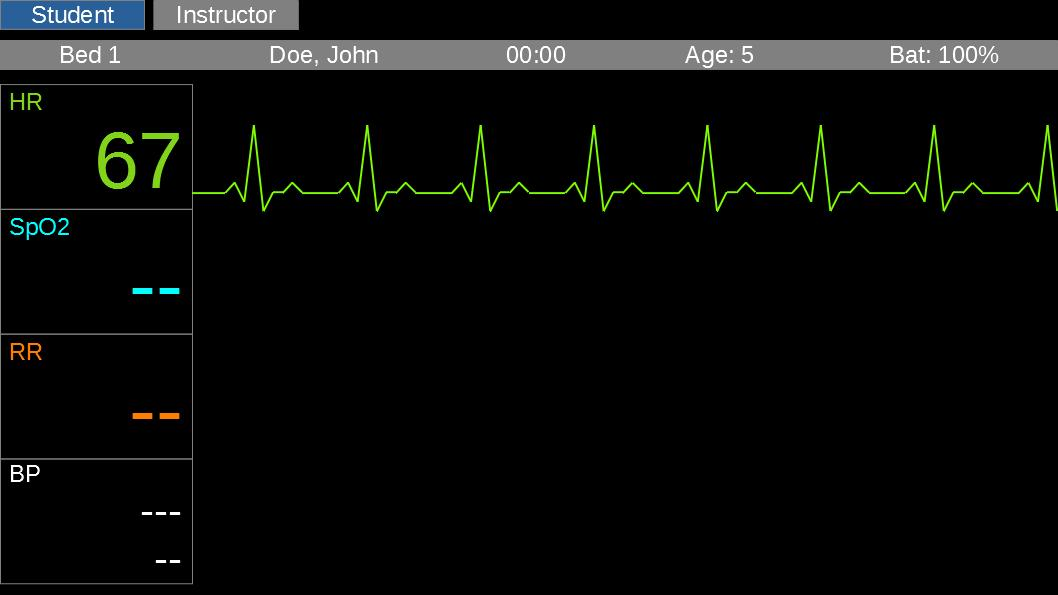
\includegraphics[scale=0.5]{gui-student}
\caption{Student GUI screen that is designed to simulate the look of an actual vital signs monitor}
\label{fig:student}
\end{figure}

This ECG signal will change at the different landmarks along the catheter's path. These landmarks are the upper, mid, and lower right atrium; upper, mid, and lower right ventricle, pulmonary artery, superior vena cava, and inferior vena cava (Objective 4). If the signal is indicating the position is at the pulmonary artery or inferior vena cava, you have missed the ventricle and should back out to try again.

Once the ECG displays the signal for the lower right ventricle (see your instructor for example of this signal), begin to pace the catheter using the pacer. The ECG will show spikes when the pacer is sending a current (User Story 6). The instructor will have set a current threshold for when the heart will polarise prior to the training exercise (User Story 5, Objective 3). If the threshold is not reached, increase the current on the pacer.

When the instructor is satisfied with student performance, the training model can be reset by removing the catheter and any medical interventions. The GUI will be reset to its original state automatically upon catheter removal.



\clearpage
\section{Appendix}

\subsection{User Stories}
The following user stories were derived from the needs presented by our client, Dr. Claudia Ranniger \cite{sprintlog}.

\begin{enumerate}
  \item Determine ECG morphology based on catheter location in the relevant vasculature region
  \item Display ECG while catheter is moving
  \item Connect catheter to pacer device to communicate location and for pacing stimulation
  \item Allow student to set pacing frequency and current
  \item Allow instructor to set pacing current threshold and initial beats per minute
  \item Determine how ECG responds to pacer settings (current and beats per minute)
\end{enumerate}


\subsection{Objectives}
The following objectives were considered in the engineering design of the device \cite{backgroundreport}.

\begin{enumerate}
  \item Be easy to interface with for the instructor
  \item Be able to display signal on trainer room monitor
  \item Be able to have the instructor set a pacing threshold (in mA and frequency)
  \item Be able to indicate to the student the current location of the catheter as they move toward RV wall
  \item Be able to illustrate physiological variability in interval duration and wave amplitudes
  \item Contain morphological accurate signals
  \item Be able to accurately determine catheter location during times of increased motion (e.g. shaking due to nervousness)
\end{enumerate}


\subsection{Functions}
The following functions were required to meet our objectives \cite{backgroundreport}.

\begin{enumerate}
  \item Detect catheter position
  \item Display a continuous ECG signal based on the location of the balloon catheter
  \item Detect and display the corresponding signal when the catheter is between two sensors
  \item Generate an ECG signal based on heart rate chosen by instructor
  \item Generate an ECG signal based on current catheter location and heart rate
\end{enumerate}

\clearpage
\bibliographystyle{ieeetr}
\bibliography{references}

\end{document}
